\documentclass{whureport}
\usepackage{float}
\usepackage{graphicx}
\usepackage{tcolorbox}
\usepackage{ctex}
\usepackage[utf8]{inputenc}

\usepackage{listings}
\usepackage{xcolor}  

\definecolor{mygreen}{rgb}{0,0.6,0}
\definecolor{mygray}{rgb}{0.5,0.5,0.5}
\definecolor{mymauve}{rgb}{0.58,0,0.82}

\begin{document}

% Front page
% 以下是标题页内容
\begin{titlepage}
\pagestyle{empty}
	\newcommand{\HRule}{\rule{\linewidth}{0.5mm}}
 \center
	
\includegraphics[width=8cm]{logo.pdf}\\[1cm] 
	\center 
	\quad\\[0.5cm]
	\textsl{\Huge 武汉大学 }\\[0.5cm] 
	\textsl{\huge 国家网络安全学院}\\[0.5cm] 
    \textsl{\LARGE 计算机网络实践实验报告}\\[0.5cm]

	\makeatletter
	\HRule \\[0.4cm]
	{ \LARGE \bfseries \ 计算机网络实践一}\\[0.4cm]
	\HRule \\[0.cm]
		\begin{center}

           \Large
            \begin{tabular}{r l}
            \textbf{姓名:} & 胡欣彤\\
            \textbf{学号:} & 2021302181178\\
            \textbf{专业:} & 网络空间安全\\
            \textbf{指导老师:} & 林海
            \end{tabular}
\begin{tabular}{c c c c c}
\textbf{其他组员:} & 查其微 & 杨雨诗 & 黄建焯 & 肖启阳
\end{tabular}
            
		\end{center}
	\makeatother
 %
\includegraphics[width=8cm]{logo.pdf}\\[1cm]
 
	{\large \textup{二〇二四年四月}}\\[2cm] 
	\vfill 
\end{titlepage}
% 标题页到此结束
\

\thispagestyle{empty}
\tableofcontents
\makeheader
\setcounter{page}{1}

% \fontsize{10pt}{12pt}\selectfont %更改段内字体字号 小四+单倍行距

% ---------------------------------------------------------------------------------
% ---------------------在下面填写内容,上面的是格式引用不要动-----------------------
% -----------------最后写完了再复制到自己的仓库里改对应的人名-----------------------
% -------------------------------------------------------------------------------
\section{实验目的及内容}
\section{实验环境}
\section{实验步骤}
\section{结果分析}
\section{出现的问题及解决方法}
\section{实验心得}

\iffalse
图片插入
\begin{figure}[H]
	\centering
	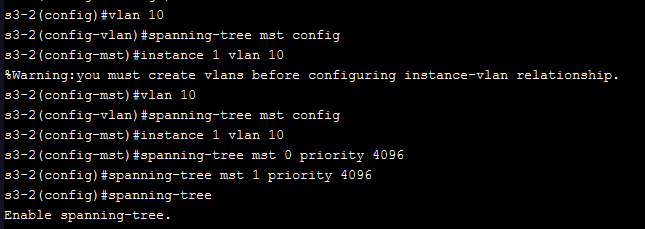
\includegraphics[width = 12cm]
	{figures/14.png}
	\caption{社交网络数据集}
	\label{data8}
\end{figure}

代码插入
\begin{python}
	class BertRe(nn.Module):
	def __init__(self, args):
	super(BertRe, self).__init__()
	self.bert = BertModel.from_pretrained(args.bert_dir)
	self.bert_config = BertConfig.from_pretrained(args.bert_dir)
	self.hidden_size = self.bert_config.hidden_size
	self.linear = nn.Linear(self.hidden_size, args.num_labels)
	self.criterion = nn.CrossEntropyLoss()
	
	def forward(self,
	input_ids,
	attention_mask,
	token_type_ids,
	labels=None):
	bert_output = self.bert(input_ids=input_ids)
	seq_out = bert_output[1]  # [batchsize, 768]
	seq_out = self.linear(seq_out)
	loss = None
	
	if labels is not None:
	loss = self.criterion(seq_out, labels.long())
	model_output = ModelOutput(seq_out, labels, loss)
	return model_output    
\end{python}
\fi
%\scriptsize\selectfont{\bibliographystyle{IEEEbib}
% \bibliography{reference}}
\small\bibliographystyle{ieeetr}
\bibliography{reference}




\newpage
\section{指导教师评语及成绩}
\noindent
【评语】
\begin{table}[H]
\centering
%\renewcommand\tablename{表}		  		% 将’Table 1'更改为'表 1'
%\setlength{\abovecaptionskip}{0pt}	 	% 自己设置caption的上间距
%\setlength{\belowcaptionskip}{5pt}		% 自己设置caption的下间距
\setlength{\tabcolsep}{7mm}			% 可以调表的总宽度
\scalebox{1}{							% 可以调整表格整体大小
\begin{tabular}{cccccccccc}
 &  &  &  &  &  &       &  &         &  \\
     &  &  &  &  &  &       &  &         &  \\
     &  &  &  &  &  &       &  &         &  \\
     &  &  &  &  &  &       &  &         &  \\
     &  &  &  &  &  &       &  &         &  \\
     &  &  &  &  &  &       &  &         &  \\
     &  &  &  &  &  &       &  &         &  \\
     &  &  &  &  &  &       &  &         &  \\
     &  &  &  &  &  & 成\quad\quad 绩:   &  & 指导老师签名: &  \\
     &  &  &  &  &  & 批阅日期: &  &         & 
\end{tabular}
}
\end{table}

\end{document}